\chapter{Experiments} \label{Experiments}

In this chapter, we define our experiment, the parameters involved in it for different agents and implementations and the final results of the simulation based on the implementation. The main focus of this chapter will be to characterize the complexity for different implementations mainly in terms of move time complexity with different implementations and the result of tournament considered between the different agents.

We first consider the implementation of the Minimax algorithm with the depth limited version, alpha-beta pruning version and the parallel version for different Quoridor board dimensions and demonstrate the time complexity of the implemented agents in terms of average move time complexity.\\
To run the experiment on all 3 implemented variants of the Minimax algorithm, we use the \textbf{Quoridor.ConsoleApp} console application, and simulate 100 games with different board and agent configurations against the semi-random strategy - a total of 36 times (3 variants of minimax x 3 depth x 4 dimensions).

For example, we use the following command line arguments to simulate 100 games between \textbf{Parallel Minimax} with a depth of 1 and \textbf{Semi-Random} agents on a game board of dimension 5x5:

\begin{lstlisting}[language=bash]
$dotnet run play -s1=parallelminimaxab -s2=semirandom -dimension=5 -depth=1 -sim -numsim=100
\end{lstlisting}

The aforementioned command produces the following output:

\begin{lstlisting}
===Results===
Player A : Parallel MinimaxAlgorithmABPruning won 99/100 games. Win rate : 99%. Average move time(ms) : 3.04
Player B : Semi-Random won 1/100 games. Win rate : 1%. Average move time(ms) : 1.05
Toal moves made across 100 games : 1781
Average total moves per game : 17
\end{lstlisting}
\\
From the result above, we see that Parallel Minimax took \textbf{1781} moves across 100 games, with an average of \textbf{3.04 ms} per move.

\begin{figure}[!ht]
    \centering
    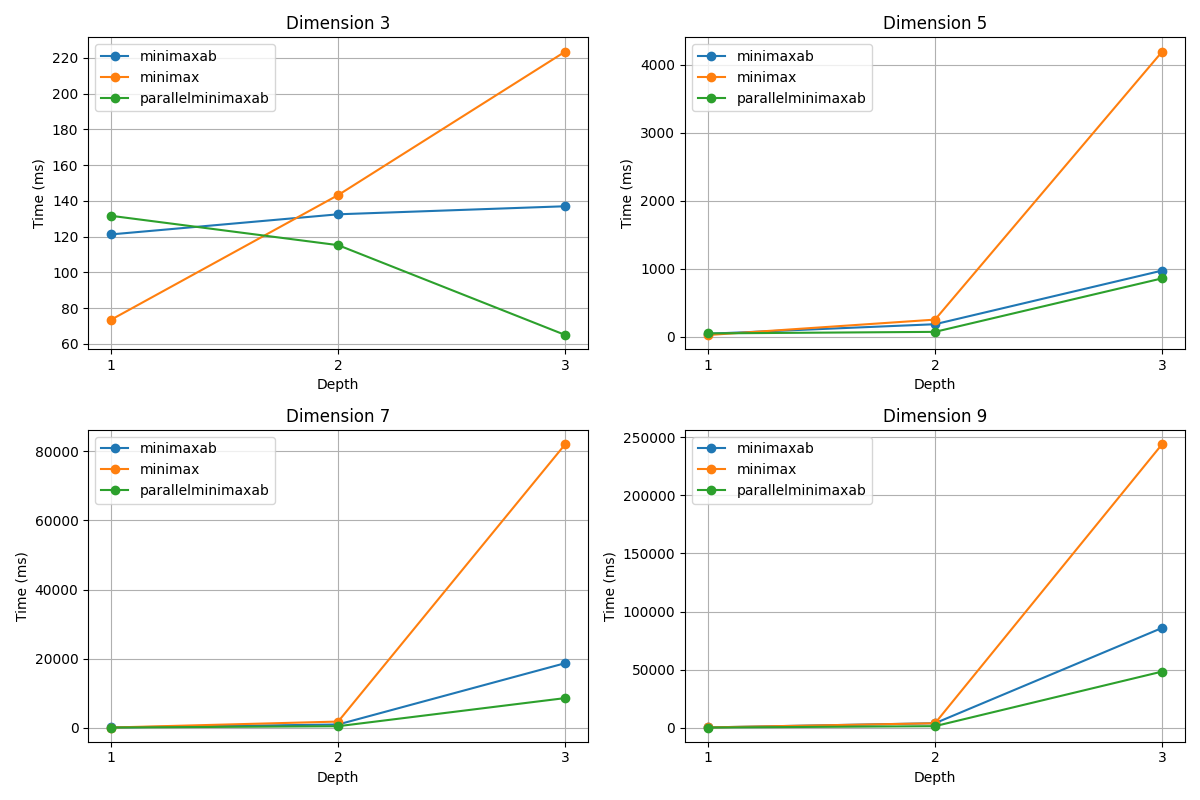
\includegraphics[width=\linewidth]{../img/performance.png}
    \caption{Average move time comparison between all 3 Minimax variants for different board sizes}
    \label{fig:minimax_performance_comp}
\end{figure}

In the figure \ref{fig:minimax_performance_comp}, we can see the average move time complexity of the implementation with different board dimension. Considering the board of large dimension (e.g., 7x7 and 9x9), without further optimization, the complexity of implementing the algorithm for Quoridor is prohibitively high. For example, for depth 3, the move time complexity for the board with dimension 7 is 82 seconds and that for dimension 9 is 244 seconds.

From the figure, it can be inferred that for depth 1, the minimax algorithm without any further optimizations including alpha-beta or parallel implementation performs the best. The reason for this is straightforward, as for depth 1, the algorithm only evaluates one further move. In such case, there is not further improvement with alpha beta as we anyways need to evaluate all the nodes. Similarly, the complexity of implementing the parallel algorithm outweighs the simple sequential evaluation.

However, for depths more than 1, it can be seen that the time complexity for each move considering alpha-beta pruning and further parallel implementation of the algorithm significantly improves as we increase the considered depth. Below, we have a table showing the improvement of the time complexity considering the minimax algorithm without any further implementation as baseline.

\begin{table}[ht]
    \centering
     \begin{tabular}{|c|c|c|c|}\hline
          & Depth 1 & Depth 2 & Depth 3\\ \hline 
          \textbf{Dimension: 3x3}  &    &    &     \\ \hline
          Minimax  &  1  &   1 &   1  \\ \hline
          Minimax alpha-beta &  1.8 &  0.92 &  0.61 \\ \hline
          Minimax alpha-beta parallel & 1.79 & 0.8& 0.29  \\ \hline
          \textbf{Dimension: 5x5}  &    &    &     \\ \hline
          Minimax  &  1  &   1 &   1  \\ \hline
          Minimax alpha-beta &  1.82 &  0.72 &  0.23 \\ \hline
          Minimax alpha-beta parallel & 2.06 & 0.27 & 0.20  \\ \hline
          \textbf{Dimension: 7x7}  &    &    &     \\ \hline
          Minimax  &  1  &   1 &   1  \\ \hline
          Minimax alpha-beta &  1.29 &  0.53 &  0.22 \\ \hline
          Minimax alpha-beta parallel & 1.05 & 0.25 & 0.10 \\ \hline
          \textbf{Dimension: 9x9} &    &    &     \\ \hline
          Minimax  &  1  &   1 &   1  \\ \hline
          Minimax alpha-beta &  1.06 &  1 &  0.35 \\ \hline
          Minimax alpha-beta parallel & 0.43 & 0.33 & 0.19  \\ \hline
     \end{tabular}
     \caption{Table with the values of relative move-time complexity compared to the baseline minimax algorithm}
     \label{tab:complexity}
 \end{table}

In the table \ref{tab:complexity}, we present the relative move time complexity of the different algorithms with reference to the minimax algorithm for the same depth. Here, we can see that, especially for depth 2 and depth 3, the time minimax algorithm when using the alpha beta pruning and further parallel implementation reduces significantly. This is significant especially when considering the large dimension of the Quoridor board as the move time complexity is significantly high. Here, optimization is required for running the algorithm in relatively manageable time.

Following, we also performed the simulations with the \gls{MCTS} agent. In the simulation, we consider a Quoridor board of dimension 5x5 \textcolor{red}{and play against a Minimax agent.}. As described in earlier sections, the \gls{MCTS} algorithm requires multiple iterations through the game tree. More iterations provide a more reliable strategy at the cost of time complexity. This is even more prominent as we increase the dimension of the board due to the exponential increase in the state space and game tree complexity as described in section \ref{GameAnalysis}.

\begin{figure}[!ht]
    \centering
    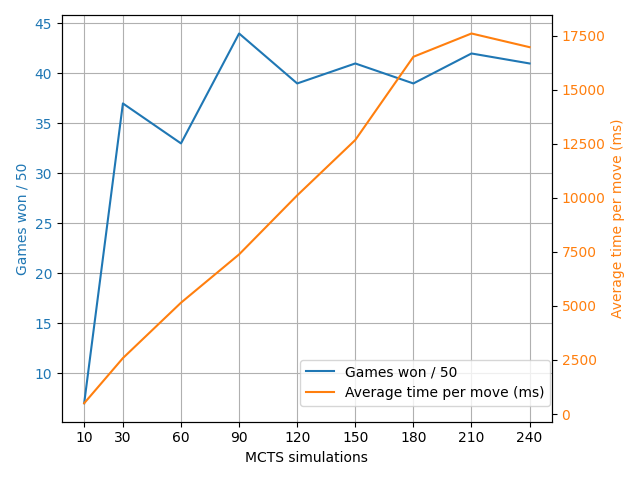
\includegraphics[width=0.7\linewidth]{../img/mcts_simulation_grid_search.png}
    \caption{Average time per move and win rates of MCTS agent with varying simulations for board size 5x5}
    \label{fig:mcts_simulations}
\end{figure}

In figure \ref{fig:mcts_simulations}, we show variation of the number of games won with the \gls{MCTS} agent againt the minimax agent varied with the number of game iterations. In the same figure, we also show the average time per move required when varying game simulations with the number of \gls{MCTS} simulations. For each number of varied \gls{MCTS} simulation, we performed 50 game simulations. We can see that after 90 simulations, the additional marginal number of game won does not increase, although the time per move increases. Hence, optimizing the number of simulations can be important to limiting the complexity of the \gls{MCTS} agent.

\begin{figure}[!ht]
    \centering
    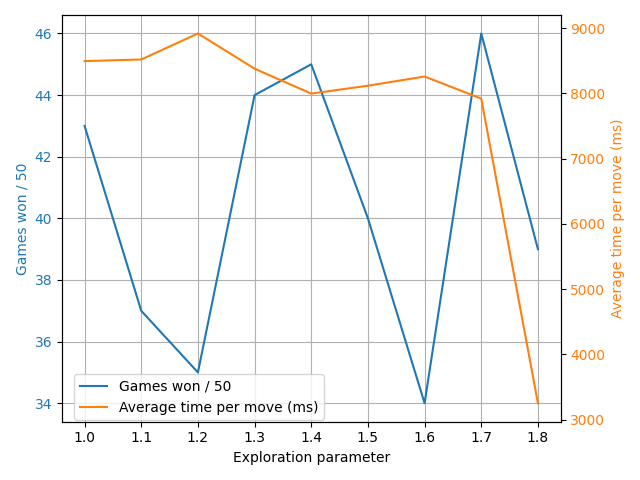
\includegraphics[width=0.7\linewidth]{../img/mcts_exploration_param_grid_search.png}
    \caption{Average time per move and win rates of MCTS agent with varying exploration parameter for board size 5x5}
    \label{fig:mcts_exp_simulations}
\end{figure}

Likewise, in figure \ref{fig:mcts_exp_simulations}, we consider find the optimal exploration parameter based on number of games won varied with different exploration parameters, In \gls{MCTS}, the exploration parameter is used in the exploration step to explore the nodes not visited yet. In addition, in the figure, we also show the average move time for different exploration parameters. In the figure, we see that with an optimal exploration parameter of 1.7 the win rate for the agent is high i.e., 46 wins out of 50 games.

\begin{table}[!ht]
    \centering
     \begin{tabular}{|c|c|c|c|c|c|}\hline
                & Random & Semi-Random & A*  & Minimax & MCTS \\ \hline 
    Random      &        &    31.3     & 6.6 &   5.3   &  0   \\ \hline
    Semi-Random &   73.5 &             & 11.5&   10.2  & 0.1  \\ \hline
    A*          &   92.2 &    90.2     &     &   0     &  0   \\ \hline
    Minimax     &   92.4 &    88.9     & 1.5 &         &  0   \\ \hline
    MCTS        &   98   &    89.3     &  16 &   3     &      \\ \hline
     \end{tabular}
     \caption{Agent comparison for dimension 3x3}
     \label{tab:agent_eval_3x3}
 \end{table}

\begin{table}[!ht]
    \centering
     \begin{tabular}{|c|c|c|c|c|c|}\hline
                & Random & Semi-Random & A*  & Minimax & MCTS \\ \hline 
    Random      &        &    5.8      &  0  &   0     &   0  \\ \hline
    Semi-Random &   93.6 &             & 0.3 &   1.9   &  3.3 \\ \hline
    A*          &   100  &    99.7     &     &   1     & 73.3 \\ \hline
    Minimax     &   92.4 &    88.9     & 1.5 &         & 33.3 \\ \hline
    MCTS        &   100  &    100      & 56.7&   92    &      \\ \hline
     \end{tabular}
     \caption{Agent comparison for dimension 5x5}
     \label{tab:agent_eval_5x5}
 \end{table}

\begin{table}[!ht]
    \centering
     \begin{tabular}{|c|c|c|c|c|c|}\hline
                & Random & Semi-Random & A*  & Minimax & MCTS \\ \hline 
    Random      &        &    2        &  0  &   0     &      \\ \hline
    Semi-Random &   99.6 &             & 0.2 &  0.7    &      \\ \hline
    A*          &   100  &    99.7     &     &   0     &      \\ \hline
    Minimax     &   100  &    99.3     & 100 &         &      \\ \hline
    MCTS        &        &             &     &         &      \\ \hline
     \end{tabular}
     \caption{Agent comparison for dimension 7x7}
     \label{tab:agent_eval_7x7}
 \end{table}

\begin{table}[!ht]
    \centering
     \begin{tabular}{|c|c|c|c|c|c|}\hline
                & Random & Semi-Random & A*  & Minimax & MCTS \\ \hline 
    Random      &        &    0        &  0  &   0     &      \\ \hline
    Semi-Random &   100  &             &  0  &  0.1    &      \\ \hline
    A*          &   100  &    100      &     &  2.8    &      \\ \hline
    Minimax     &   100  &    100      & 100 &         &      \\ \hline
    MCTS        &        &             &     &         &      \\ \hline
     \end{tabular}
     \caption{Agent comparison for dimension 9x9}
     \label{tab:agent_eval_9x9}
 \end{table}
 